\documentclass{article}
\usepackage{graphicx}
\usepackage{amsmath,amssymb,amsthm}
\usepackage{color}
\usepackage{fullpage}

\def\xcolorversion{2.00}
\def\xkeyvalversion{1.8}

\usepackage[version=0.96]{pgf}
\usepackage{tikz}
\usetikzlibrary{arrows, backgrounds, positioning, fit, shapes, automata, shadows}
\usepackage[latin1]{inputenc}

\DeclareMathOperator*{\argmax}{arg\,max}
\DeclareMathOperator*{\argmin}{arg\,min}

\usepackage[backref,pageanchor=true,plainpages=false, pdfpagelabels, bookmarks,bookmarksnumbered]{hyperref}

\begin{document}

\title{De Novo Variant Caller using Google Genomics API}

\author{
	Subhodeep Moitra\\ 
	Carnegie Mellon University \\
	{\tt subhodee@cs.cmu.edu}
}

\maketitle

\begin{abstract}
This tool identifies de novo genetic mutations in a family trio (child, mother and father). De novo genetic mutations are defined as those mutations which occur in the child but do not occur in the genomes of the parents. This tool queries the Google Genomics API in order to search and retrieve genetic variants and reads. It implements a Bayesian inference algorithm for identifying  de novo mutations from the retrieved data. This document describes theory, design and early experiments for the de novo caller. 
\end{abstract} 

\section{Background}
De novo genetic mutations are a set of rare genetic mutations that occur in the genomes of a child but do not occur in the genome of the child's parents. These mutations are being increasingly implicated to play an important role in a variety of diseases such as Autism~\cite{Michaelson2012} and Schizophrenia. With the advent of Whole Genome Sequencing, a large number of these mutations are being discovered at both the exonic and the intronic regions. 

\vspace{1em}
Detecting de novo mutations is a challenging task. Some of the issues that affect de novo mutation detection are : 
\begin{itemize}
\item \textbf{Rare event}: A de novo mutation is a very rare event ($\sim$1 in $10^8$ bp).
\item \textbf{Sequencing errors}: Sequencing errors occur at the rate of 1 in 100 bp. This makes it much more likely to observe a sequencing error rather than a de novo mutation.
\item \textbf{Read Depth}: Since the reads mapped to a particular position are essentially random, it is possible that the denovo mutation is completely skipped by inadequate coverage at that position.
\item \textbf{Misalignment}: Variant detection pipelines assume a high quality alignment of reads. In areas of poor alignment, variant detection suffers.
\item \textbf{Expensive Validation}: Candidates have to be verified through expensive Sanger sequencing.
\item \textbf{Structural Variation}: Complications arise through structural variations in the chromosome through insertions, deletions, inversions, copy number variations, translocations, etc.
\end{itemize}

The Google Genomics API~\cite{GoogleGenomics} provides services to import and query variants and reads data. This tool assumes that variants and reads are available for the trio under study and have been imported into the Genomics API. The tool provides two callers (1) Variant Caller (2) Read Caller. The variant caller walks over the trio of genomes and examines SNPs avaiable through the \verb|variants| API. After filtering for variants based on quality cutoffs and mendelian inheritance rules, a set of candidate calls are generated and passed onto the Read Caller for finer discrimination. The Read Caller makes requests to the \verb|reads| API to fetch mapped reads for these candidate position and makes a finer call using a bayesian inference algorithm.  Validation experiments against NA12878 trio from Platinum genomes~\cite{platinum} were also run and compared against experimentally validated de novo and somatic mutations~\cite{Conrad2011} ; results are reported in section ~\ref{experiments}.

\subsection{Bayes Net}
We employ a probabilistic inference framework using bayes nets for de novo variant calling. A bayes net belongs to the class of mathematical models known as graphical models which are a marriage between graph theory and probability theory~\cite{Jordan2008}. A Bayes Net is a directed acyclic graph which defines conditional independence relationships between random variables in a probability distribution. A Bayes net can be used for sampling, marginal inference and decoding of the hidden variables. 

\begin{figure}
\centering
\begin{tikzpicture}[->,>=stealth',shorten >=1pt,auto,node distance=2.8cm,
                    semithick]
  \tikzstyle{parent}=[circle,thick,draw=blue!75,fill=blue!20,minimum size=6mm]
  \tikzstyle{child}=[parent,draw=red!75,fill=red!20]
  \tikzstyle{data}=[rectangle, copy shadow, thick,draw=black!75,
  			  fill=black!20,minimum size=4mm]

  \node[child] 		   (C)                    {$G_C$};
  \node[parent]         (F) [above left of=C] {$G_F$};
  \node[parent]         (M) [above right of=C] {$G_M$};
  \node[data]         (DC) [below of=C] 		{$D_M$};
  \node[data]         (DF) [below of=F]       {$D_F$};
  \node[data]         (DM) [below of=M]       {$D_C$};

  \path (F) edge              node {} (C)
            edge              node {} (DF)
        (M) edge              node {} (C)
            edge              node {} (DM)
        (C) edge              node {} (DC);
        
\end{tikzpicture}
\caption{The hidden variables $G_{F}, G_{M}$ and $G_{C}$ correspond to the genotypes of the father, mother and child respectively. The genotypes take one among 10 values from $AA, AC, AT, AG, CC, CT, CG, GG, GT$ and $TT$. The trio of genotypes values can thus have $10^3$ possible values. The observed variables ($D_F, D_M$ and $D_C$) are the bases present at the candidate position for a particular read }
\label{fig:bayesnet}
\end{figure}

\vspace{5mm} 
We follow the bayes net implementation for de novo variant calling as in Li et al~\cite{Li2012}. They model a bayes net to encode the diploid Mendelian relationship between the members of the trio. See Figure~\ref{fig:bayesnet} for an illustration of the bayes net. The hidden variables $G_{F}, G_{M}$ and $G_{C}$ correspond to the genotypes of the father, mother and child respectively. The genotypes take one among 10 values from $AA, AC, AT, AG, CC, CT, CG, GG, GT$ and $TT$. The trio of genotypes values can thus have $10^3$ possible values. The observed variables ($D_F, D_M$ and $D_C$) are the reads obtained at a candidate position. We fix the baseline sequencing error rate $\epsilon_{seq}$ and the baseline de novo mutation rate $\epsilon_{denovo}$. In equation~\ref{eqn:model}, we apply Bayes rule to calculate the probability of a particular genotype trio given observed reads.

\begin{equation}\label{eqn:model}
P(G_F,G_M,G_C|D_F,D_M,D_C) =  \frac{P(D_F,D_M,D_C|G_F,G_M,G_C)P(G_F,G_M,G_C)}{\sum_{G_F,G_M,G_C}P(D_F,D_M,D_C|G_F,G_M,G_C)P(G_F,G_M,G_C)}
\end{equation}

\noindent 
The term $P(D_F,D_M,D_C|G_F,G_M,G_C)$ is the data likelihood and is calculated as in equation~\ref{eqn:read_likelihood}. 

\begin{align}\label{eqn:read_likelihood}
P(D_F,D_M,D_C|G_F,G_M,G_C) &= P(D_F|G_F)P(D_M|G_M)P(D_C|G_M) \\
	&= \left(\prod_{f=1}^{|D_F|}P(R_f|G_F)\right)\left(\prod_{m=1}^{|D_M|}P(R_m|G_M)\right)\left(\prod_{c=1}^{|D_C|}P(R_c|G_C)\right)
\end{align}

\noindent
The term $P(G_F,G_M,G_C)$ encodes the mendelian inheritance relationship in the trio and can be factorized further according to equation~\ref{eqn:mendel_factor}. Furthermore, this likelihood can be expressed in terms of $\epsilon_{seq}$ and $\epsilon_{denovo}$ as in equation~\ref{eqn:mendel_likelihood} where $N_{denovo}$ corresponds to the number of $G_C$ cases that are de novo given the parents ; similarly $N_{mendelian}$ corresponds to the number of $G_C$ cases that are mendelian given the parents.

\begin{equation}\label{eqn:mendel_factor}
P(G_F,G_M,G_C) = P(G_C|G_F,G_M)P(G_F)P(G_M)
\end{equation}

\begin{equation}
\label{eqn:mendel_likelihood}
 P(G_C|G_F,G_M) = \left\{ 
  \begin{array}{l l}
    \epsilon_{denovo}/N_{denovo} & \quad \text{if $G_C$ is a denovo mutation}\\
    (1-\epsilon_{denovo})/N_{mendelian} & \quad \text{otherwise}
  \end{array} \right.
\end{equation}

\vspace{1em}
The base likelihood $P(R|G)$ conditioned on the genotype of the sample is calculated according to equation~\ref{eqn:base_likelihood}.

\begin{equation}
\label{eqn:base_likelihood}
P(R|G) = \left\{ 
  \begin{array}{l l}
    1-\epsilon_{seq} & \quad \text{if $G$ is homozygous and $R \in G$}\\
    \epsilon_{seq}/3 & \quad \text{if $G$ is homozygous and $R \notin G$}\\    
      0.5(1-2\epsilon_{seq}/3) & \quad \text{if $G$ is heterozygous and $R \in G$}\\
    \epsilon_{seq}/3 & \quad \text{if $G$ is heterozygous and $R \notin G$}
  \end{array} \right.
\end{equation}
  
\subsection{Bayesian Inference Strategies}
In the previous section we defined the bayes net model. In this section we will discuss the inference strategies for determining if a candidate position is a de novo variant. We define the function $I_{denovo}(G_F,G_M,G_C)$ as an indicator function when the child genotype is a de novo mutation. We also calculate the likelihoods of all the de novo and the mendelian inheritance cases as described in equation~\ref{eqn:denovo_like}.

\begin{align}
\label{eqn:denovo_like}
L_{denovo} &= \sum_{G_F,G_M,G_C}P(D_F,D_M,D_C|G_F,G_M,G_C)P(G_F,G_M,G_C)I_{denovo}(G_F,G_M,G_C)\\
L_{mendelian} &= \sum_{G_F,G_M,G_C}P(D_F,D_M,D_C|G_F,G_M,G_C)P(G_F,G_M,G_C)I_{mendelian}(G_F,G_M,G_C)
\end{align}

\subsubsection{Maximum A Posteriori (MAP)} 
Call a de novo variant if condition~\ref{eqn:map} holds.
\begin{equation}
\label{eqn:map}
I_{denovo}(\argmax_{G_F,G_M,G_C} P(G_F,G_M,G_C|D_F,D_M,D_C))
\end{equation}

\subsubsection{Bayesian Risk Minimizer (Bayes)} 
Call a de novo variant if condition~\ref{eqn:bayes} holds. This inference rule minimizes the empirical bayesian risk.

\begin{equation}
\label{eqn:bayes}
\frac{L_{denovo}}{L_{denovo} + L_{mendelian}} > 0.5
\end{equation}

\subsubsection{Likelihood Ratio Test (LRT)} 
Call a de novo variant if condition~\ref{eqn:lrt} holds where $\mathcal{T}$ is a user specified likelihood ratio threshold. Note that LRT is the same as Bayes if $\mathcal{T}$ is equal to $1$.

\begin{align}
\label{eqn:lrt}
\frac{L_{denovo}}{L_{mendelian}} > \mathcal{T}
\end{align}

\section{Design and Implementation}

\begin{figure}
\centering
\begin{tikzpicture}[->,>=stealth',shorten >=1pt,auto,node distance=3cm,thick,
  pleasure node/.style={circle,fill=red!20,draw,font=\sffamily\bfseries},
  blank node/.style={circle,fill=blue!20,fill opacity=0,font=\sffamily\bfseries}]
  \tikzstyle{files}=[rectangle, copy shadow, thick,draw=black!75,
  			  fill=black!20,minimum size=8mm]


	\tikzstyle{bucket}=[draw, fill=blue!20, minimum height=6em, minimum width=8em, cylinder, shape border rotate=90, thick, shape aspect=0.1]

  \tikzstyle{component}=[rectangle, draw=black!75, fill=yellow!20,minimum size=8mm]

 \tikzstyle{rectsplit} = [   
        align=center,                                           
        draw,
        rectangle split,
        rectangle split horizontal,
        rectangle split parts=3
    ]

\begin{scope}

    \node [bucket] (Vs)                                    {\textbf{Varstore}};
    \node [bucket, fill=red!20] (Rs) [below of=Vs, yshift=-4cm]                      {\textbf{Readstore}};
    \node [files] (V) [left of=Vs, fill=blue!20, xshift=-1cm]                                   
    {\begin{tabular}{c}
    \textbf{Variants}\\
	\small{.VCF files}
     \end{tabular}};
    \node [files] (R) [left of=Rs, fill=red!20, xshift=-1cm]                      {\begin{tabular}{c}
    \textbf{Reads}\\
	\small{.BAM files}
     \end{tabular}};


\node[component,    	% layout (defined above)
  right of=Vs, 	% Position is to the right of QUERY
  xshift=2.5cm] (VStr) 	
 { Variant Stream};
 
\node[component,    	% layout (defined above)
  right of=VStr, xshift=1.2cm] (VBuf) 	
 { Variant Buffer};

\node[component,    	% layout (defined above)
  below of=VBuf, yshift=1cm] (MFil) 	
 { Mendel Filter};

\node[component, fill=green!20, copy shadow,   	% layout (defined above)
  below of=MFil, yshift=0.8cm] (filt) 	
 { Filtered Candidates};


\node[component,    	% layout (defined above)
  right of=Rs, 	% Position is to the right of QUERY
  xshift=2.5cm] (RStr) 	
 { Read Stream};
 
\node[component,    	% layout (defined above)
  right of=RStr, xshift=1.2cm, minimum height=1cm, minimum width=4cm, align=center] (Binf) 	
{\emph{Bayesian Inference}\\[2em]};

\node[rectsplit, align=center] at (Binf)
       (inf)
       {      \nodepart{one}
          \textbf{MAP} \nodepart{two}
          \textbf{Bayes} \nodepart{three}
          \textbf{LRT}};
          
\node[component, fill=green!80, copy shadow,     	% layout (defined above)
  below of=Binf, yshift=0.7cm] (final) 	
 { Final Candidates};

\node[component, minimum height=1mm, fill=black!20, xshift=0.5cm, yshift=0.4cm, draw=black!10] at (Binf.north west) (Rcall) 	
 { \textbf{Read Caller}};

\node[component, minimum height=1mm, fill=black!20, xshift=-0.7cm, yshift=0.4cm, draw=black!10] at (VBuf.north west) (Vcall) 	
 { \textbf{Variant Caller}};


 \path[every node/.style={font=\sffamily\small}]
    (V) edge node [below] {$import$} (Vs)
    (R) edge node [above]   {$import$} (Rs)
    (Vs) edge node [above]   {API Calls} (VStr)
    (VStr) edge node    {} (Vs)
    (Rs) edge node [above]   {API Calls} (RStr)
    (RStr) edge node  {} (Rs)
    (VStr) edge node [above] {Buffering} (VBuf)
    (RStr) edge node [above] {} (Binf)
    (VBuf) edge node [right] {} (MFil)
    (MFil) edge node [right] {} (filt)
    (filt) edge node [right] {} (Binf)
    (filt) edge node [right] {} (RStr)
    (Binf) edge node [right] {} (final);
    
\end{scope}

  \begin{pgfonlayer}{background}
    \filldraw [line width=4mm,join=round,black!10]
      (Vcall.north  -| VStr.west)  rectangle (MFil.south  -| MFil.east)
      (Rcall.north  -| RStr.west)  rectangle (Binf.south  -| Binf.east);
  \end{pgfonlayer}
\end{tikzpicture}
\caption{ De novo variant caller design : There are two main components (1) Variant Caller interacting with Varstore (2) Read Caller interacting with Readstore. The Variant caller makes API calls to Varstore using a Variant Stream object that interfaces with a variants buffer. The buffer manages overlapping variants from the trio. Once a set of suitable variants have been obtained it is filtered using mendelian inheritance checks. These candidates are then passed onto the the Read Caller which obtains reads for the candidate position from readstore. The candidates are filtered using one of three Bayesian inference procedures (1) MAP - Maximum a posteriori (2) Bayes Rule (3) LRT - Likelihood Ratio test. Successful candidates are written onto disk.}
\label{fig:design}
\end{figure}

This tool is designed as a standalone command line tool for performing inference. This tool assumes that variants and reads are available for the trio under study and have been imported into the Genomics API. 

\vspace{1em}
There are two main components (1) Variant Caller interacting with Varstore (2) Read Caller interacting with Readstore. See Figure~\ref{fig:design} for an illustrative diagram. The Variant caller makes API calls to Varstore using a Variant Stream object that interfaces with a variants buffer. The buffer manages overlapping variants from the trio. Once a set of suitable variants have been obtained it is filtered using mendelian inheritance checks. These candidates are then passed onto the the Read Caller which obtains reads for the candidate position from readstore. The candidates are filtered using one of three Bayesian inference procedures (1) MAP - Maximum a posteriori (2) Bayes Rule (3) LRT - Likelihood Ratio test. Successful candidates are written onto disk.

\subsection{Concurrency / Multi-threading}
Profiling indicated that a lot of time was spent in network I/O delays. To speed up the execution, requests to the \verb|variants| API and the \verb|reads| API can be parallelized using multiple threads. Performance testing showed that multi-threading achieves a linear speedup with the number of threads(Graphs not shown). For this purpose the Variant Caller and the Read Caller implements a helper class \verb|SimpleDenovoRunnable| and \verb|BayesDenovoRunnable| respectively. Their behavior can be controlled by the \verb|--num_threads| option.


\subsection{Commandline usage}
This tool is predominantly meant to be used from the commandline.

\subsubsection*{Typical commandline use}
See below for typical commandline usage : 

\begin{verbatim}
java -jar target/denovo-variant-caller-0.1.jar --caller full \
--client_secrets_filename ${HOME}/Downloads/client_secrets.json \
--dataset_id 14004469326575082626 \
--dad_callset_name NA12891 \
--mom_callset_name NA12892 \
--child_callset_name NA12878 \
--chromosome chr1 \
--start_position 1 \
--end_position 14000000 \
--log_level debug \
--num_threads 25 \
--output_file NA12878_full.calls
\end{verbatim}


\subsubsection*{All options}
See below for all available options:

\begin{verbatim}
Usage: DenovoMain [flags...]
 --caller [VARIANT | READ | FULL]       : The caller mode
 --child_callset_name <name>            : Child's callset name e.g. NA12879
 --chromosome <name>                    : specify the chromosomes to search
                                          (specify multiple times for multiple
                                          chromsomes)
 --client_secrets_filename <file>       : Path to client_secrets.json
 --dad_callset_name <name>              : Dad's callset name e.g. NA12877
 --dataset_id <id>                      : Dataset id
 --denovo_mut_rate <rate>               : Specify the denovo mutation rate
                                          (default 1e-8)
 --end_position <position>              : end position ( usually set
                                          automatically )
 --inference_method [MAP | BAYES | LRT] : Inference method (map | bayes | lrt)
 --input_calls_file <file>              : File to read from
 --log_file <file>                      : specify the log file
 --log_level [ERROR | INFO | DEBUG]     : specify the logging level
 --lrt_threshold <sig_level>            : likelihood ratio test significance
                                          level (default 1. ;higher the
                                          stricter)
 --max_api_retries <num>                : max api retry count (default 5)
 --max_variant_results <num>            : max variants returned per request
                                          (default 10000)
 --mom_callset_name <name>              : Mom's callset name e.g. NA12878
 --num_threads <num>                    : Specify the number of threads
                                          (default 1 ; 1 to 50 suggested)
 --output_dir <dir>                     : File to write results
 --output_file <file>                   : File to write results
 --seq_err_rate <rate>                  : Specify the sequence error rate
                                          (default 1e-2)
 --start_position <position>            : start position ( usually 1 )
\end{verbatim}


\section{Experiments}
\label{experiments}
We ran validation experiments against the NA12878 trio (NA12878 child, NA12891 father, NA12892 mother) from Platinum genomes~\cite{platinum} and compared them against experimentally validated de novo and somatic mutations~\cite{Conrad2011}. The results are shown in Table~\ref{tab:NA12878}. The tool has high recall $\sim 96\%$. The precision is less than desirable ; however it is only a lower bound since the NA12878 trio is derived from cell lines and hence has accumulated a lot of somatic cell mutations. A blood line dataset may reveal more accurate numbers. The compute time is favorable ; 3 hours to go over 3 Billion base pairs. 

\vspace{1em}
Figure~\ref{fig:variant_caller} shows a false de novo mutation  candidate at chr10:23,662,774 in NA12878 trio. The top two tracks correspond to parents (NA12891 and NA12892) while the bottom track (NA12878) corresponds to the child genome. Father Genotype from \verb|variants| API is $AA$, mother genotype is $AA$ while child is $AG$. Variant is called by variant caller but correctly rejected by read caller due to insufficient evidence from reads. The Bayesian inference reads caller observes that there have been occurrences of some $G$ bases in the parents which diminishes the likelihood of a denovo mutation.

\vspace{1em}
Figure~\ref{fig:germline} shows a true experimentally validated germline mutation at chr1:75,884343 in NA12878 trio. The top two tracks correspond to parents (NA12891 and NA12892) while the bottom track (NA12878) corresponds to the child genome. Inferred father Genotype is $TT$, mother genotype is $TT$ while child is $CT$. De novo mutation is called correctly by both variant and read caller. 

\begin{table}
    \label{tab:NA12878}
    \centering
    \begin{tabular}{ | c | c | c | c | c | c |}
    \hline
    \textbf{Filter} & \textbf{Num Calls Filter} & \textbf{Precision} & \textbf{Recall }& \textbf{Time} & \textbf{Throughput} \\ \hline
	Variant & 4090 & 22.12\%* & 96.69\% & $\sim$3 hours (20 threads) & $\sim$3 mbps(20 threads) \\\hline
	Variant $+$ BayesNet & 2207 & 40.55\%* & 95.62\% & $\sim$30 mins(20 threads) & $\sim$ 1.5 mbps
(20 threads) \\
    \hline
    \end{tabular}
    \caption{Results on NA12878 trio (NA12878 child, NA12891 father, NA12892 mother) from Platinum genomes~\cite{platinum} compared against experimentally validated de novo and somatic mutations~\cite{Conrad2011}. The tool has high recall $\sim 96\%$. \textit{* The precision is inconclusive ; most likely is a lower bound since the NA12878 trio is derived from somatic cell lines. A follow up blood line experiment will likely reveal more accurate numbers.} The compute time is favorable; 3 hours to go over 3 Billion base pairs. }
\end{table}

\begin{figure}[!ht]
  \centering
  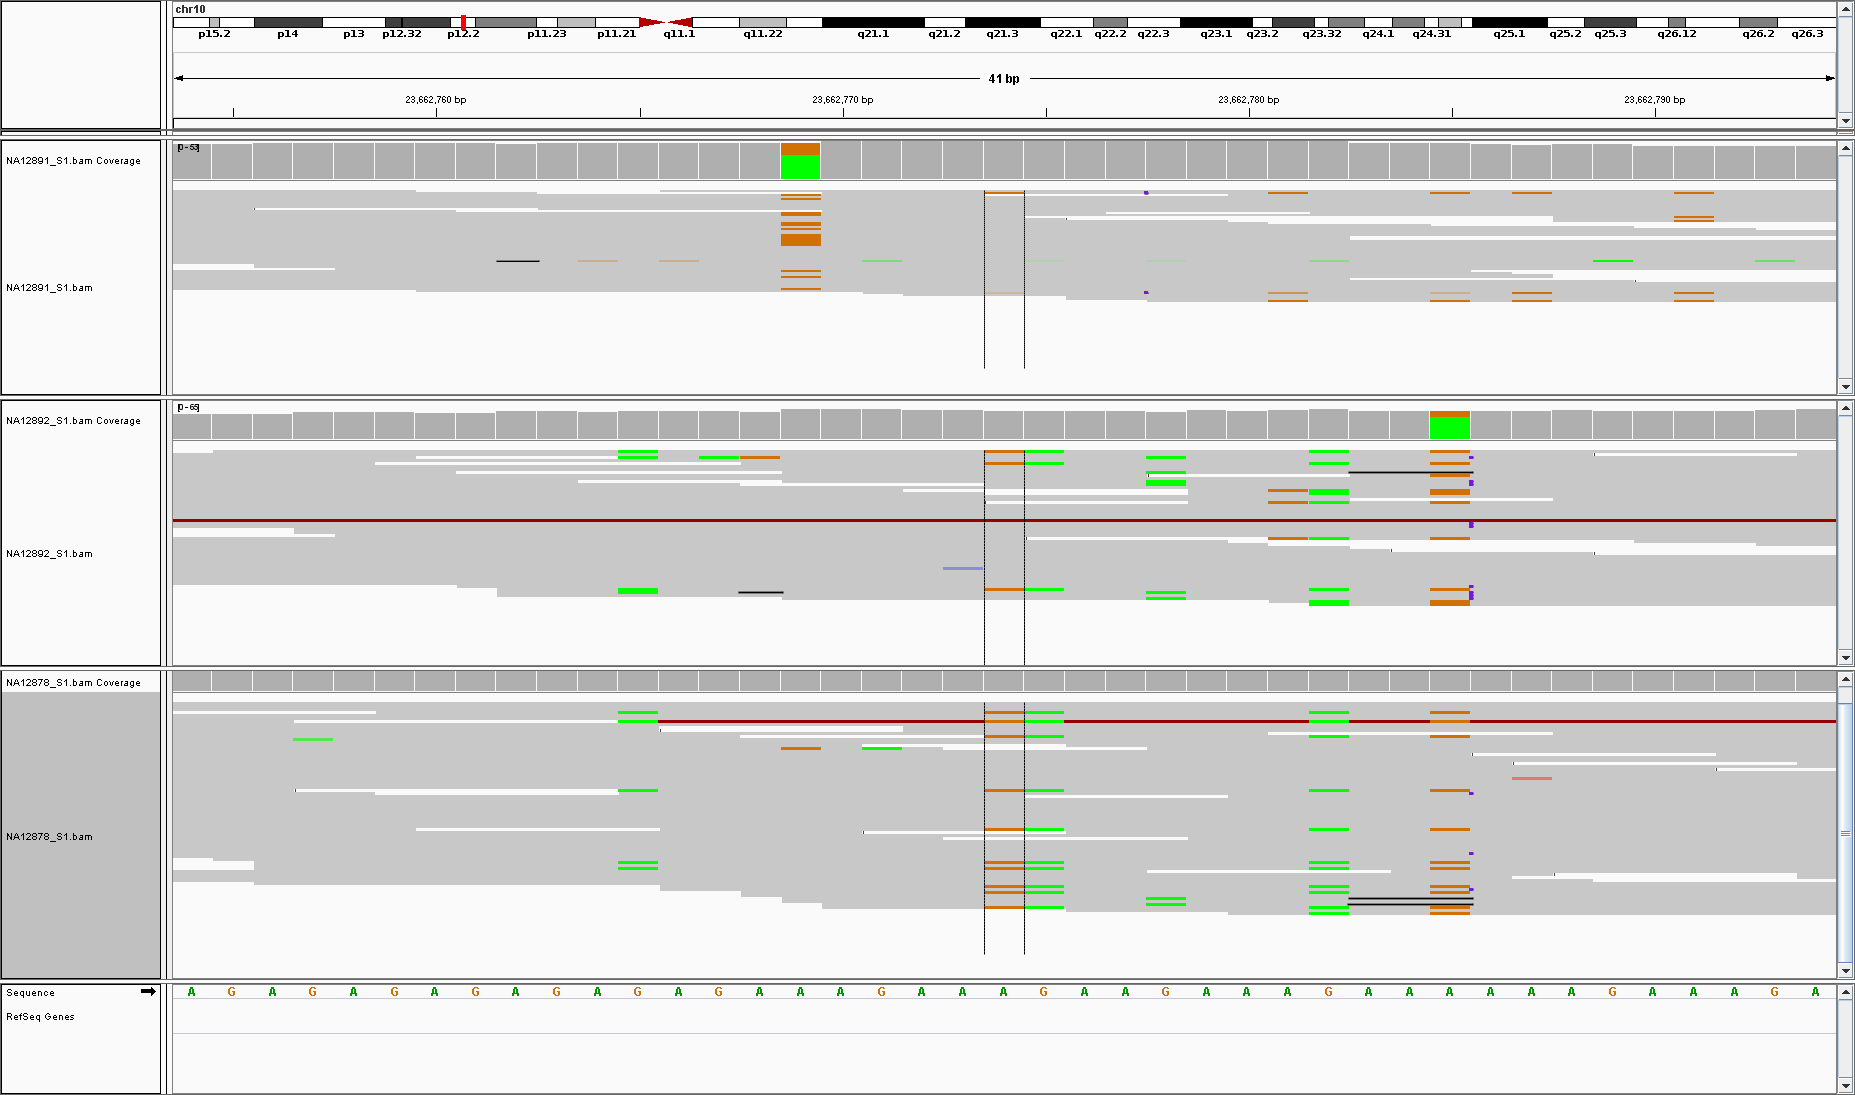
\includegraphics[width=6in]{chr10_23662774.png}
  \caption{Shows a false candidate for a denovo mutation at chr10:23662774 in NA12878 trio. The top two tracks correspond to parents (NA12891 and NA12892) while the bottom track corresponds to the child genome (NA12878). Father Genotype variant is $AA$, mother genotype is $AA$ and child is $AG$. Variant is called by variant caller but correctly rejected by read caller due to insufficient evidence from reads. The bayesian inference reads caller observes that there have been occurrences of some $G$ bases (brown lines) in the parents which diminishes the likelihood of a denovo mutation.}
   \label{fig:variant_caller}
\end{figure}


\begin{figure}[!ht]
  \centering
  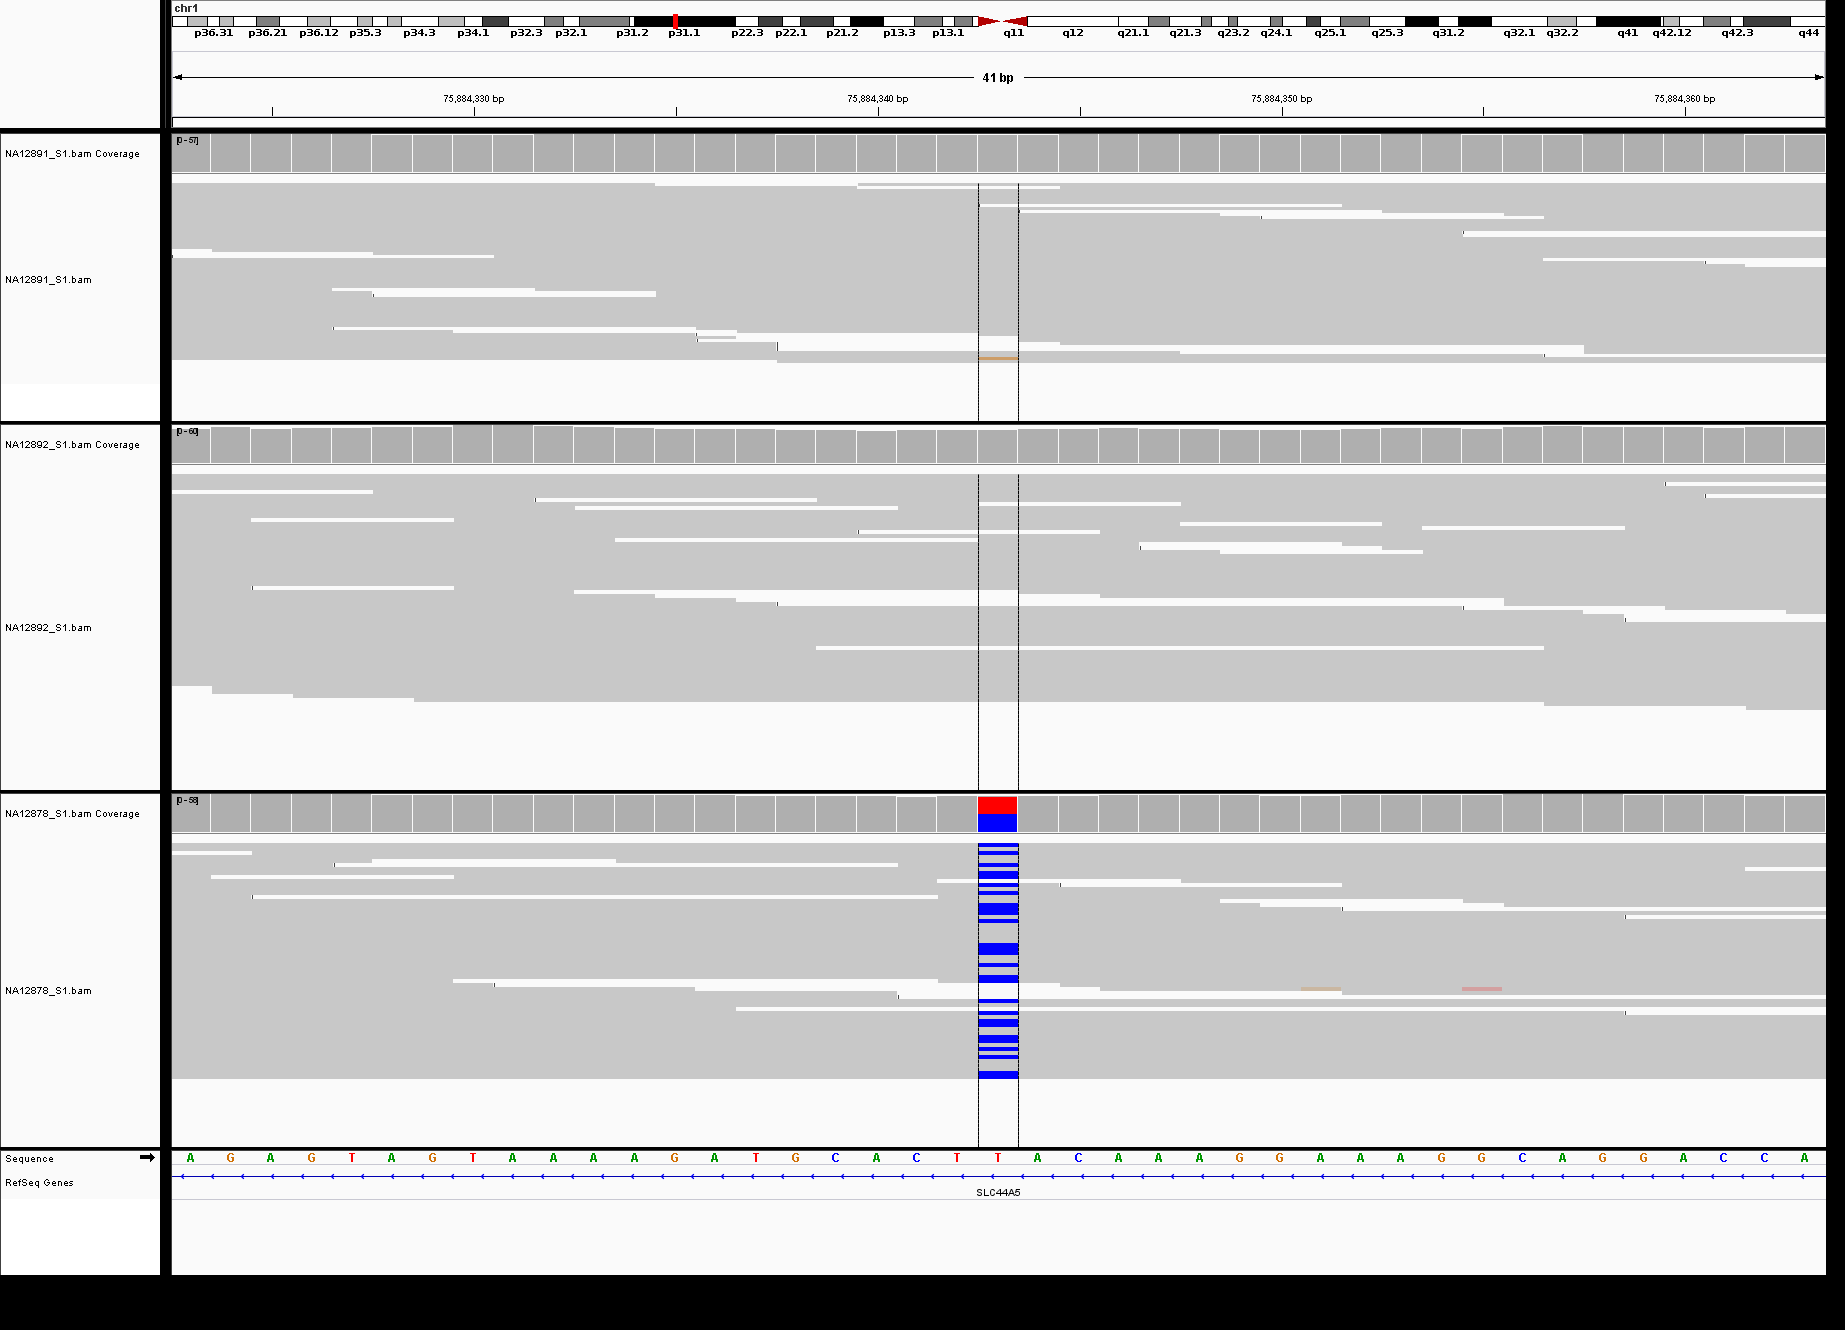
\includegraphics[width=6in]{chr1_75,884,323_75,884,363.png}
  \caption{Shows a true experimentally validated germline mutation at chr1:75,884343 in NA12878 trio. The top two tracks correspond to parents (NA12891 and NA12892) while the bottom track (NA12878) corresponds to the child genome. Inferred father Genotype is $TT$, mother genotype is $TT$ while child is $CT$. Variant is called by correctly by both variant and read caller}
   \label{fig:germline}
\end{figure}


\section{Future Work and Conclusion}
This tool identifies de novo genetic mutations in a family trio (child, mother and father) by exercising the Google Genomics API to fetch variants and reads which is subsequently  . It provides concurrency options to speed up execution. Experiments were run against the NA12878 trio which showed high recall $\sim 96\%$ against experimentally validated germline and cell line mutations. Precision scores were inconclusive and will need follow up experiments against blood derived genomes.


\begin{thebibliography}{10}

\bibitem{Li2012}
   Li B et. al,
   \emph{A likelihood-based framework for variant calling and de novo mutation detection in families},
   PLoS Genetics, 2012
   Volume 8, Number 10, Pages e1002944

\bibitem{Michaelson2012}   
   Michaelson et al,
   \emph{Whole-Genome Sequencing in Autism Identifies Hot Spots for De Novo Germline Mutation},  
   Cell, 2012, 
   Volume 151, Number 7, Pages 1431 - 1442

\bibitem{Jordan2008}
	Wainwright, Jordan,
	\emph{Graphical Models, Exponential Families, and Variational Inference},
	Foundations and Trends in Machine Learning, 2008,
	Volume 1, Issue 1-2, pp 1-305	

\bibitem{Conrad2011}
	Conrad et al., 
	\emph{Variation in genome-wide mutation rates within and between human families},
	Nature Genetics, July 2011
	Volume 43, Number 7, pp 712-715

\bibitem{GoogleGenomics}
	\emph{Google Genomics API},
	\url{https://developers.google.com/genomics/}

\bibitem{platinum}
	\emph{Platinum Genomes - Illumina Sequencing},
	\url{http://www.illumina.com/platinumgenomes/}
	
\end{thebibliography}
\end{document}